\chapter{Introduction}

% Trends of the electronic field is size reduction
Integrated circuits miniaturization continues nowadays allowing increasingly massive integration of electronic functions.
Size reduction is accomplished by decreasing integrated technology feature size.
An integrated technology defines the dimensions and processes required to manufacture an integrated circuit and its fundamental conception bricks.
The main characteristic of a technology is the feature size called \textlambda{} that represents the smallest dimension for a transistor gate.
All other dimensions of the technology are defined as an integer multiplication factor of \textlambda{}.
The value of \textlambda{} determines the size, power consumption, switching speed, performance and many other properties of the complete chip.
Until recently, Moore's law successfully predicted that technology dimensions will be reduced by a factor of two every 18 months.
The automotive world follows this trend as well, moving recently to \SI{16}{\nano\metre} technology nodes (see Fig. \ref{fig:nxp-techno-increase}) \cite{evolution_technologies} that are normally employed in less demanding applications.

% Benefits of size reduction
Reduction of \textlambda{} results in more massive integration on a given silicon surface.
The area occupied by a function on silicon is the main cost factor.
Reducing this area allows to diminish the unit manufacturing cost resulting in increased profits and margins.
For the same area, integrated circuits in more recent technologies can pack more functionalities with higher performances.
Weight reduction of electronic modules in automotive or aerospace lowers fuel consumption, and reduces the impact on the environment.

\begin{figure}[!h]
  \centering
  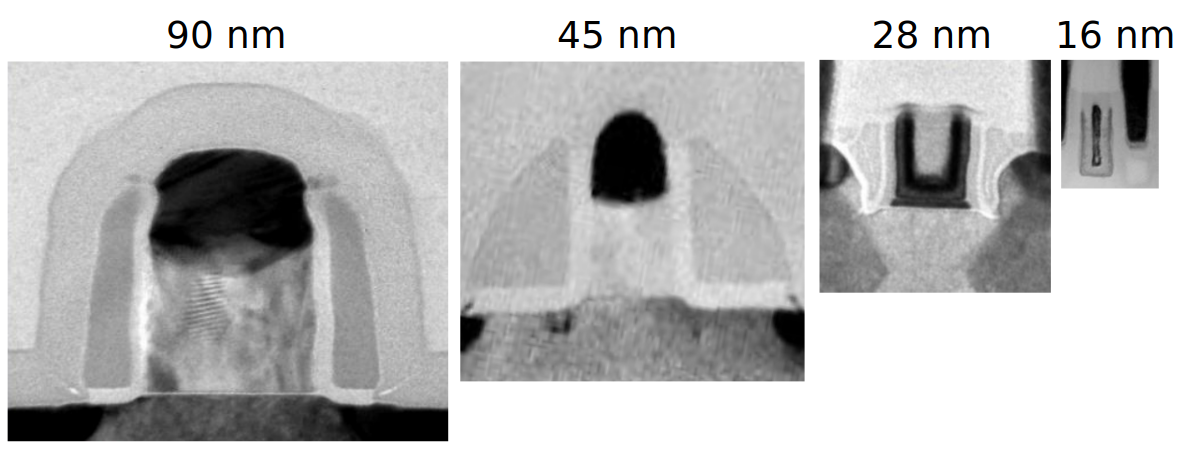
\includegraphics[width=\textwidth]{src/1/figures/technology_evolution.pdf}
  \caption{Recent evolution of NXP's automotive technology nodes \cite{evolution_technologies}}
  \label{fig:nxp-techno-increase}
\end{figure}

% Side effects of size reduction
The decrease of \textlambda{} results in reduction of insulating material's thickness.
Transistor gate oxide becomes thinner, tolerating smaller differences of potential before breakdown.
After breakdown, the oxide starts leaking significant amount of currents and the transistor becomes unusable.
As a result, the technology provides more sensitive conception bricks and a larger silicon area must be dedicated to protecting the core circuitry \cite{evolution_technologies}.

% Another trend in automotive - more electronic functions
New major trends are also emerging in the automotive field.
The development of fully autonomous driving is seeing tremendous progress.
This class of functionalities take decisions and perform critical actions such as braking or steering the wheel.
Those features are developed to offer increased safety for the user.
A side consequence is that electronic modules now have very high responsibilities.
The real-time constraint is particularly important, meaning that electronic circuits must perform their duties with no delay and operate correctly all the time.
For instance, an airbag system must always be ready to trigger in case of car accident without any delay.
Electric cars raise new challenges for safety as well, such as battery management.
Those features require more computing power, more sensing capabilities and more data to exchange.
As a consequence, the amount of \gls{ecu}s and electronic modules in a car is growing quickly.
Communication buses like the \gls{can} \cite{CAN} or \gls{lin} \cite{LIN} are shared by multiple systems and new standards appear for supporting higher bandwidths.
The CAN bus with Flexible Data rate (CAN-FD) is an example of this trend.

% Harsh environment in the automotive field
The automotive environment is quite harsh for electronic devices and equipments are exposed to a wide range of stresses.
A running engine generates plenty of vibrations and mechanical stress.
A lot of heat and thermal cycling is produced when the engine is on, and a vehicle is exposed to large temperature variations during its lifetime.
Electrical contacts, solder joints and connections suffer from these stresses, and must be designed to withstand them.
Electronic system are also exposed to a wide range of electrical stresses especially in the automotive field.
Transient disturbances can be generated by natural phenomena or by the vehicle itself.
When the engine is turned on, the battery voltage can drop very low due to the amount of current drawn by the ignition.
This voltage drop can affect electronic systems and damage them.
Another major source of electrical stress is called the \gls{esd}.

% What is an ESD
An electrostatic discharge is the sudden flow of electricity between two objects of different charge.
It is the result of a local accumulation of electrostatic potential.
When a large enough potential difference is reached, a very rapid and violent discharge occurs.
It is common to record amplitudes in the range of thousands of volts and tens of amperes.
A study by Renault car manufacturer \cite{Renault-esd} estimates that electronic devices are exposed 10000 times to \gls{esd}s during their lifetime.
It has always been considered a very serious threat for electronic systems.

% Architecture systemes automobiles
In terms of architecture, a vehicle is constituted by a multitude of electronic modules interconnected by cables.
Interconnected electronic systems need to share a good ground reference for them to communicate and work properly.
The car's metallic body is the ground reference for all electronic modules, because a good connection to Earth is impossible inside a vehicle.
Electronic modules and the battery are all linked to the car's body using wires and cables.
In \gls{dc} and at low frequencies, this ground connection is good because the vehicle's body is a very large chunk of metal with a very low resistance.
At high-frequencies though, those cables have an inductive behavior.
They oppose to variations of currents and exhibit large potential differences.
Local disturbances can shift the ground reference between one module an another.
Electrostatic discharges are high frequency events of very large amplitude and can cause disturbances like this.
Inside a vehicle, the discharges can propagate inside cables by conduction, or by coupling between cables through radiated emission.
Electronic modules are designed to be robust but the complex architecture and the very violent nature of ESD makes challenging to guarantee immunity.

\begin{figure}[!h]
  \centering
  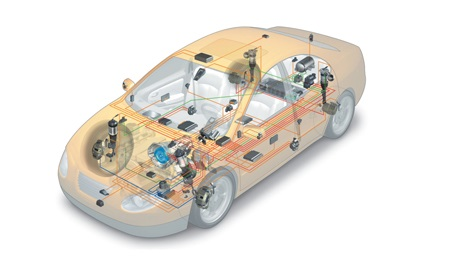
\includegraphics[width=0.7\textwidth]{src/1/figures/systemintegration_01_uv-data.jpg}
  \caption{Architecture of electronic systems in a vehicle \cite{car-architecture}}
  \label{fig:car-architecture}
\end{figure}

% Fiabilite vis a vis des ESD
In summary, electronic devices must operate in severe automotive environment while using more sensitive conception bricks.
Despite the robustness of modules, disturbances such as electrostatic discharges can cause failures.
In the \gls{esd} field, there are two kinds of failures to consider.
The hardware failure, or hard-failure, is when an electronic device is permanently damaged \cite{impactESDsemiconductors}.
Destruction can occur through oxide breakdown, when a voltage too large is applied on an insulating material.
It can also occur through thermal breakdown, when current through a structure is too high and causes a meltdown.
Two examples of failures can be observed in Fig. \ref{fig:esd-failures}).
Recently, a new class of failures is being studied.
Soft-failure, or functional failure, is when an electronic device fails temporarily to perform its function, because of an electrical disturbance.
Different levels of severity can be identified depending on the impact of the failure on the rest of the system.
A module that is momentarily disturbed by a discharge but recovers immediately is less severe than a module that requires user intervention.
Also, failures on the airbag system are much more severe than on the entertainment system, because user safety is put at risk in the first case.
A first article on the topic was published by F. Caignet and N. Lacrampe in 2007 \cite{LacrampeTransientImmunity}.
A large amount of research at the system level was published in EOS/ESD symposium 2012 \cite{soft-error-esd-1,SDRAMCase,mixedModeESDSims} and 2013 \cite{softFailSubsystem, powered-tlp-soft-fail}.
The draft standard IEC 62433-6 \cite{iec62433-6} aims to provide a base framework for soft-failures analysis and prediction.
Analysis of the literature reveals that most studies are currently focused on system-level soft-failure analysis.
There is currently no real work at the component level or studies performed inside the design of an integrated circuit.

\begin{figure}[!h]
  \centering
  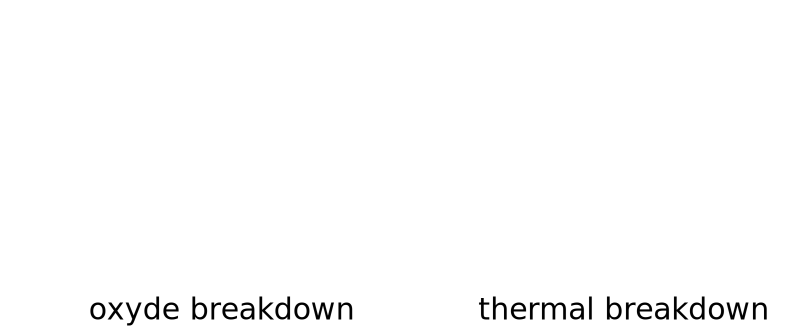
\includegraphics[width=\textwidth]{src/1/figures/esd_failures.pdf}
  \caption{Different kinds of ESD-induced failures (Credit: \cite{phd-monnereau})}
  \label{fig:esd-failures}
\end{figure}

% Conception methods
Beyond studying failures inside integrated circuits, it is important to keep in mind how chips are designed and developed.
This is important to propose solutions that are actually implementable.
This entire process from the specification to the manufacturing of a product is called the design flow.
During this process, there are many teams and people involved.
Modeling team creates electrical model of technology components.
Design team assembles component together to create integrated functions that conform to the specification.
Layout team translates the symbolic view of electrical netlists into the series of masks and layers required by manufacturing.
The laboratory tests manufactured parts and runs investigations in case of failures.
The \gls{esd} and \gls{emc} team has the particularity to interact will all teams because issues and solutions can be found in any step of the design flow.
Overall, the integrated circuits are designed hierarchically and the flow is a bottom-up process.
Fundamental bricks are assembled together in rising complexity to create the required functions.
The main source of delay in this process is the manufacturing time which can be of several months.
Designs are put on silicon but the parts are tested only after manufacturing, several months later.
To gain time to market and be competitive, it is essential to reduce to a bare minimum the amount of design-manufacturing-testing cycles.
Each additional manufacturing is very expensive, and increases further the development time of the product.
This is why any simulation tool able to predict early any kind of failure (and functional failures among them) is very valuable for silicon design companies.

% What is provided in this document
It was demonstrated that real-time electronic circuits have higher responsibilities yet they can be disturbed by disturbances such as electrostatic discharges.
Also, most studies on the topic of functional failure due to \gls{esd} are focused on system-level analysis.
In this document, research and analysis of functional weaknesses is done lower in the electronic system hierarchy, at the integrated circuit level.
It is essential to understand how failures appear in order to fix them and prevent them prior to manufacturing.
For this purpose, many approaches and methods are proposed in this document.
A modeling method of electronic systems exposed to electrostatic discharge is developed, improving prior work on the topic \cite{phd-lacrampe, phd-monnereau}.
It allows to determine what fraction of an incoming discharge actually reaches the integrated circuit.
Then, on-chip measurement methods have been designed and manufactured, in order to acquire more data inside the chip.
Those methods comprise monitoring devices such as an on-chip current sensor, overvoltage and undervoltage detectors, and a communication chain for fast prototyping.
Finally, modeling methods were experimented using simulation tools.
The first method models each block function individually, then offer to chain and combine models together to deduce the robustness of a complete top-level function.
The second method aims to build an electrical equivalent model of the integrated circuit, for system-level simulations.
Black box modeling that abstract the internal design using only the external behavior is used.
Finally, a concept of an assertion system is detailed, to identify quickly and efficiently during preliminary design phase the potential weakness of an integrated circuit.

\begin{figure}[!h]
  \centering
  \includegraphics[width=\textwidth]{src/1/figures/overview_flow.pdf}
  \caption{Highly simplified integrated circuit design flow - specification, symbolic view, layout, silicon}
  \label{fig:ic-design-flow}
\end{figure}

% Presentation des chapitres
%
Chapter \ref{chap:1} details what is an electrostatic discharge and how to reproduce it in laboratory conditions.
This preliminary work highlights how functional failures appear and how they impact electronic devices.
The literature about ESD-induced soft-failures is reviewed .
It is demonstrated that so far that most of the studies are focused at the system level, and that it remains very challenging to identify failure root cause without access to the chip design.

%
Chapter \ref{chap:2} presents a modeling method for simulating \gls{esd} waveforms up to the integrated circuit inputs.
The first challenge for understanding soft-failures at silicon-level is to determine what fraction of an incoming \gls{esd} actually reaches the integrated circuit.
Between the injection point of a stress and the disturbed circuit, many devices are connected such as cables, discrete devices, etc.
Each element interacts with the discharge, absorbs a part of its current or changes the waveform.
A model library of common electrical elements found in \gls{esd} testing environment has been constructed and is detailed.
The modeling method is applied to a complex pulse generator, and yields a highly accurate model.
Finally, a new test generator was developed to overcome some issues met during the debug of silicon-level failures using system level \gls{esd} testers \cite{iec61000-4-2, iso10605}.
The principle of operation and architecture of the generator is described.
It produces the same compliant waveform than those standards, with some advantages such as increased testing reproducibility and zero radiated emission.

%
A case of soft-failure in an integrated circuit is explained in chapter \ref{chap:3}.
In a first phase, measurement data is obtained at the board level and the failure is explained.
Simulations are run to understand how failures appear, and more specifically how a short electrical event can disturb an integrated circuit for a long period of time.
In a second phase, the integrated function is placed onto a custom testchip.
Specific on-silicon structures were designed to gather measurement data on electrical nets that are not physically accessible.
All these measurements are performed for the purpose of estimating the accuracy of integrated circuit \gls{esd} simulations.
There are two main potential sources of error that are checked.
Silicon technology device models are not designed to function for extremely fast transient transient disturbances.
Also, standard simulations do not take parasitic devices into account, such as metal track resistances and parasitic couplings.
Measurement data is confronted to simulations in order to verify the validity of models.
Analysis of the failure led to the development of a testchip, to put on silicon the same failing function but with a more convenient environment for measurement and investigation.

%
When issues are discovered late in the testing lab, analysis is performed manually, by trial and error, searching inside the design why the function is failing.
It is a complex and time-consuming process.
The core research of this work focuses on proposing new analysis methods and tools for electrical simulations.
It is detailed in chapter \ref{sec:methods-operating-esd-analysis}.
The first method offers to study and model block functions individually, then connect the models together to deduce the robustness of a top-level function.
The second method targets system-level simulations comprising integrated circuit.
It focuses on modeling an integrated function with a behavioral model that is not aware of the internal design, in order to run powered ESD simulations.
Finally, a concept is presented for easing the search of soft-failures during integrated circuit development.
It is based on using a assertions inside the blocks to efficiently and quickly find which function or net is being disturbed due to an ESD.

%
The conclusion in chapter \ref{sec:final-conclusion} summarizes the work achieved during the PhD, highlights the most notable discoveries, and identifies follow-up work and research topics that could be worth pursuing.
